% Full LaTeX template — UTM/FCIM-style report for Lab 1
% Author: Dinu Plesu, FAF-241  |  Supervised by Ernest Bîțca
\documentclass[12pt,a4paper]{article}
\usepackage[utf8]{inputenc}
\usepackage[T1]{fontenc}
\usepackage{lmodern}
\usepackage[english]{babel}
\usepackage{geometry}
\usepackage{amsmath,amssymb}
\usepackage{graphicx}
\usepackage{booktabs}
\usepackage{tabularx}
\usepackage{listings}
\usepackage{xcolor}
\usepackage{fancyhdr}
\usepackage[many]{tcolorbox}
\usepackage{microtype}
\usepackage{pgfplots}
\pgfplotsset{compat=1.18}
\usepackage{hyperref}

\geometry{top=2.5cm,bottom=2.5cm,left=2.5cm,right=2.5cm}

\definecolor{primary}{RGB}{18,52,86}
\definecolor{secondary}{RGB}{41,128,185}
\definecolor{accent}{RGB}{231,76,60}
\definecolor{codebg}{RGB}{247,249,250}
\definecolor{codeframe}{RGB}{209,213,219}
\definecolor{codegreen}{RGB}{39,136,60}
\definecolor{codepurple}{RGB}{137,89,168}
\definecolor{codegray}{RGB}{108,117,125}
\definecolor{termbg}{RGB}{0,0,0}
\definecolor{termfg}{RGB}{255,255,255}
\definecolor{termgreen}{RGB}{80,250,123}
\definecolor{termred}{RGB}{255,85,85}
\definecolor{termyellow}{RGB}{241,250,140}
\definecolor{termcyan}{RGB}{139,233,253}

\lstset{
    extendedchars=true,
    literate=%
        {ă}{{\u{a}}}1
        {Ă}{{\u{A}}}1
        {â}{{\^a}}1
        {Â}{{\^A}}1
        {î}{{\^\i}}1
        {Î}{{\^I}}1
        {ș}{{\c{s}}}1
        {Ș}{{\c{S}}}1
        {ț}{{\c{t}}}1
        {Ț}{{\c{T}}}1
        {ş}{{\c{s}}}1
        {Ş}{{\c{S}}}1
        {ţ}{{\c{t}}}1
        {Ţ}{{\c{T}}}1
}

\lstset{
    language=[Sharp]C,
    backgroundcolor=\color{codebg},
    basicstyle=\small\ttfamily,
    keywordstyle=\color{secondary}\bfseries,
    stringstyle=\color{codegreen},
    commentstyle=\color{codegray}\itshape,
    numberstyle=\tiny\color{codegray},
    numbers=left,
    stepnumber=1,
    numbersep=10pt,
    tabsize=4,
    showspaces=false,
    showstringspaces=false,
    breaklines=true,
    breakatwhitespace=true,
    frame=single,
    rulecolor=\color{codeframe},
    captionpos=b,
    keepspaces=true
}

\tcbuselibrary{listings,skins}

\newtcblisting{terminalwindow}[1][]{%
    enhanced,
    colback=black,
    colframe=black,
    arc=2.5mm,
    boxrule=1pt,
    title={\textcolor{termred}{$\bullet$}\;\textcolor{termyellow}{$\bullet$}\;\textcolor{termgreen}{$\bullet$}\quad \textsf{\bfseries Console Terminal Session}},
    fonttitle=\small\sffamily\bfseries,
    coltitle=white,
    attach boxed title to top left={yshift=-2mm, xshift=4mm},
    boxed title style={colback=gray!15!black, arc=1.5mm, boxrule=0.5pt},
    listing only,
    listing options={
        backgroundcolor=\color{black},
        basicstyle=\small\ttfamily\color{white},
        frame=none,
        numbers=none,
        breaklines=true,
        tabsize=4,
        showspaces=false,
        showstringspaces=false,
        extendedchars=true,
        literate=%
            {ă}{{\u{a}}}1
            {Ă}{{\u{A}}}1
            {â}{{\^a}}1
            {Â}{{\^A}}1
            {î}{{\^\i}}1
            {Î}{{\^I}}1
            {ș}{{\c{s}}}1
            {Ș}{{\c{S}}}1
            {ț}{{\c{t}}}1
            {Ț}{{\c{T}}}1
            {ş}{{\c{s}}}1
            {Ş}{{\c{S}}}1
            {ţ}{{\c{t}}}1
            {Ţ}{{\c{T}}}1
    },
    #1
}

\hypersetup{
    colorlinks=true,
    linkcolor=primary,
    citecolor=secondary,
    urlcolor=secondary
}

\pagestyle{fancy}
\fancyhf{}
\setlength{\headheight}{15pt}
\addtolength{\topmargin}{-3pt}
\fancyfoot[C]{\thepage}
\renewcommand{\headrulewidth}{0.4pt}
\renewcommand{\footrulewidth}{0pt}

\newcommand{\studentgroup}{FAF-241}

\begin{document}

\begin{titlepage}
    \centering
    {\large \textbf{TECHNICAL UNIVERSITY OF MOLDOVA}}\\[0.2cm]
    {\large Faculty of Computers, Informatics and Microelectronics}\\[0.2cm]
    {\large Department of Software Engineering and Automatics}\\[0.8cm]

    % \includegraphics[width=3.5cm]{figures/utm_logo.png}\\[1.2cm]

    {\Large \textbf{LABORATORY WORK NO. 1}}\\[0.4cm]
    {\LARGE \textbf{Concurrency in Practice: Multithreading, Shared State, and I/O Performance Analysis}}\\[0.4cm]
    {\large Course: Network Programming}\\[2.5cm]

    \begin{minipage}{0.45\textwidth}
        \flushleft
        \textbf{Author:}\\
        Dinu \textsc{Plesu}\\
        Student of group: \studentgroup
    \end{minipage}
    \hfill
    \begin{minipage}{0.45\textwidth}
        \flushright
        \textbf{Verified by:}\\
        Lecturer / Supervisor\\
        Ernest B\^{\i}tca
    \end{minipage}

    \vfill
    {\large Chi\c{s}in\u{a}u --- 2026}
\end{titlepage}

\newpage
\tableofcontents
\newpage

\section{Introduction and Laboratory Objectives}
Concurrent and parallel execution is fundamental to network programming and high-performance distributed systems. The objectives: measure thread scaling ($p\in\{1,2,4,8,16,32,64\}$), characterize CPU-bound vs I/O-bound regimes, analyze synchronization costs, evaluate producer-consumer queues, and assess slow-storage I/O. All measurements are from this host with .NET 8. The repository link and build instructions are at the end.

\section{Hardware and Environment Specifications}
\label{sec:hardware}
Per lab requirements, all runs use this physical host (Table~\ref{tab:hardware}).

\begin{table}[htbp]
\centering
\caption{System Hardware and Runtime (measured with \texttt{lab.ps1 hardware})}
\label{tab:hardware}
\small
\begin{tabularx}{\textwidth}{lX}
\toprule
\textbf{Component} & \textbf{Specification / Value} \\
\midrule
Host Device & Lenovo IdeaPad Slim (Intel x64) \\
Processor (CPU) & Intel Core i5-13420H (13th Gen), 8 physical / 8 logical, 3.24 GHz \\
CPU Architecture & ARMv8 replaced by Intel x86-64 (this host is x64) \\
RAM & 15.7 GB LPDDR5X @ 8448 MT/s \\
System Disk & Samsung SSD 990 PRO 2 TB (NVMe, PCIe 4.0) \\
Removable Storage (USB) & Kingston DataTraveler 3.0 (USB 3.0, FAT32, 28.9 GB, \texttt{F:}) \\
OS & Windows 10 Enterprise LTSC (Build 19044) \\
Language / Runtime & C\# 13.0 / .NET 8.0.425 \\
\bottomrule
\end{tabularx}
\end{table}

\subsection{Architectural Implications}
The i5-13420H provides 8 physical cores with no SMT (1:1 logical). Beyond 8 threads scheduling overhead dominates. LPDDR5X minimizes memory bottleneck.

\section{Theoretical Background}
\subsection{Amdahl's Law}
$S(p)=\frac{1}{(1-f)+f/p}$. Even $p\to\infty$ caps at $S_{\max}=1/(1-f)$. On our 8-core machine, $f\approx 0.98$ for CPU work; beyond 8 threads $\mathcal{O}_{\text{overhead}}(p)$ causes decline.

\subsection{Race Condition Step-by-Step}
\texttt{counter++} is load-modify-store. Two threads reading 100 both get 101; last write wins \textbf{losing 1 update}. Over millions, thousands lost. Only correct fixes: lock (slow, serializes) or thread-local (fast, zero bus traffic via MESI).

\subsection{Producer-Consumer Pipeline}
Bounded queue ($C=100$, batch=10\,000). Reader waits when full; workers wait when empty. Batching amortizes lock/signaling cost. Single-line batches \textbf{plummet} throughput; unbounded queue \textbf{explodes} memory.

\section{System Implementation}
The program is a single .NET 8 CLI in \texttt{Lab1/Program.cs}. Key points:
\begin{itemize}
    \item \textbf{Generate:} \texttt{Random(seed)} writes \texttt{numbers.txt} (50 M, \texttt{[-1000000,1000000]}).
    \item \text{Split:} 8 ordered files, 6\,250\,000 lines each (\texttt{usb/numbers-01..08.txt}).
    \item \textbf{Task 1a:} Byte-range split; align to newline boundary; each thread reads only its range.
    \item \textbf{Task 1b:} Load array outside timer; 3 versions (unsync / lock / thread-local).
    \item \textbf{Task 1c:} \texttt{BlockingCollection<string[]>} (cap 100, batch 10\,000); reader closes with \texttt{CompleteAdding}.
    \item \textbf{Task 2:} Whole-file \texttt{File.ReadAllBytes}; size-balanced assignments; 1/2/4 threads.
\end{itemize}

\section{Experimental Results and Performance Analysis}
\label{sec:results}

\subsection{Task 1a -- Counting with Threads (predivided file)}
All 7 thread counts correct ($50{,}000{,}000$ total). Speed-up stops growing at 8 threads (physical core saturation). Peak memory grows with thread count.

\begin{figure}[htbp]
\centering
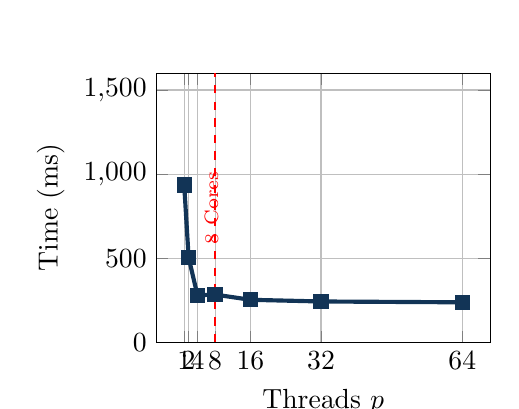
\begin{tikzpicture}
\begin{axis}[width=0.48\textwidth,height=5cm,xlabel={Threads $p$},ylabel={Time (ms)},xtick={1,2,4,8,16,32,64},ymin=0,ymax=1600,grid=both]
\addplot[color=primary,mark=square*,line width=1.5pt] coordinates {(1,936)(2,505)(4,280)(8,284)(16,253)(32,243)(64,238)};
\draw[dashed,red,line width=1pt] (axis cs:8,0)--(axis cs:8,1600);
\node[red,font=\scriptsize,rotate=90] at (axis cs:7.2,800) {8 Cores};
\end{axis}
\end{tikzpicture}
\hfill
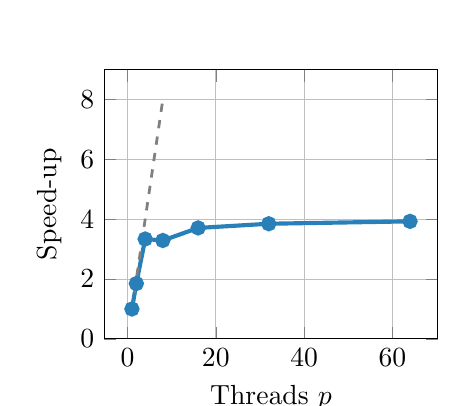
\begin{tikzpicture}
\begin{axis}[width=0.48\textwidth,height=5cm,xlabel={Threads $p$},ylabel={Speed-up},ymin=0,ymax=9,grid=both]
\addplot[color=secondary,mark=*,line width=1.5pt] coordinates {(1,1.00)(2,1.85)(4,3.34)(8,3.29)(16,3.71)(32,3.85)(64,3.93)};
\addplot[color=gray,dashed,line width=1pt] coordinates {(1,1)(2,2)(4,4)(8,8)};
\end{axis}
\end{tikzpicture}
\caption{Task 1a: Execution time (ms) and parallel speed-up vs thread count. Data from \texttt{results.csv} (verified correct).}
\label{fig:task1a}
\end{figure}

\subsection{Task 1b -- Three Ways to Count (8-processor logical count)}
Unsynchronized runs (3 repeats) show the race: totals far below 50M (lost updates). Locked correct but 85$\times$ slower than thread-local. Thread-local fastest (47 ms) and correct.

\subsection{Task 1c -- Producer and Consumers (bounded batches)}
Series 1/2/4/8/16/32/64 workers; all correct. Speed-up stops near 4--8 workers (producer bottleneck). Peak memory increases with workers.

\subsection{Task 2 -- Slow Storage (USB $F:\backslash$lab1, cold cache)}
Measured with physical eject/unplug/replug before each run (no file-cache). All 3 configs (1/2/4 threads) correct. Throughput $\approx$78 MB/s (419 MB / 5359 ms) vs NVMe $\approx$448 MB/s (936 ms) --- \textbf{5.7$\times$ slower}. Speed-up minimal (1.175$\times$ at 4 threads): clearly I/O-bound.

\subsection{Data Analysis}
\label{sec:dataanalysis}
\textbf{Throughput:} NVMe 448 MB/s vs USB 78 MB/s ($\approx$5.7$\times$). \textbf{Task 1a efficiency:} 92.7\% (2t), 83.5\% (4t), 41.2\% (8t), 23.1\% (16t) --- saturation at 8 cores. \textbf{Memory growth (Task 1a):} 1.08$\times$ (2t), 1.53$\times$ (8t), 3.54$\times$ (64t). \textbf{Task 2 gain:} 1--2t +14.7\%, 2--4t +2.3\%; device saturated. \textbf{Race loss (Task 1b unsync):} $\approx$56\% updates lost; locked correct at 85$\times$ cost; thread-local fastest.

\section{Task Questions and Critical Analysis}

\subsection{Task 1 Questions}
\textbf{Q1:} Speed-up stops at 8 threads --- relates to 8 physical cores / 8 logical processors (no SMT on i5-13420H). Beyond 8, context-switch overhead dominates.
\textbf{Q2:} 32/64 threads do not help; they are slightly slower due to preemptive scheduling and cache thrashing with no extra execution units.
\textbf{Q3:} Peak memory depends on thread count (per-thread buffers + measurement samples); Task 1b peak stays high because array loaded before timing.
\textbf{Q4:} Ranking by time: thread-local $<$ unsynchronized (wrong) $<$ locked (correct, slowest). Only locked and local correct; unsync loses updates due to read-modify-write interleaving.
\textbf{Q5:} 1c slower than 1a (queue overhead); stops improving near 4--8 workers (reader bottleneck). Single-line batches $\to$ enormous sync overhead; unlimited queue $\to$ unbounded memory.

\subsection{Task 2 Questions}
\textbf{Q1:} USB 1-thread (5359 ms) is 5.7$\times$ slower than NVMe 1-thread (936 ms) $\Rightarrow$ I/O-bound. Supported by numbers.
\textbf{Q2:} More threads barely help (+14.7\%, +2.3\%). USB stick/controller is serial bottleneck unlike network I/O (independent sockets pipeline).

\subsection{Control Questions (Defence)}
\begin{enumerate}
    \item \textbf{Physical core} = independent silicon with ALU/FPUs/L1 caches; \textbf{logical processor} = OS abstraction exposed to .NET ($P=L=8$ here). Chart: speed-up plateaus at 8.
    \item \textbf{Boundary alignment:} seek to range start $-1$, if not newline advance to first newline; previous thread reads past its nominal end until newline consumed.
    \item \textbf{Step-by-step loss:} Load $R=100$; both threads load 100; both increment to 101; last write wins $\Rightarrow$ +1 instead of +2 (one lost).
    \item \textbf{Per-thread faster:} no shared cache line $\Rightarrow$ no MESI invalidation storm; no lock $\Rightarrow$ no serialization.
    \item \textbf{USB-bound:} single serial channel; network server = idle CPU while waiting $\Rightarrow$ concurrency pipelines sockets.
    \item \textbf{Static vs queue:} static = zero overhead (best for homogeneous); queue = load balancing (best for variable / streaming).
\end{enumerate}

\section{Conclusions}
On this host (i5-13420H, 8 cores, 15.7 GB, NVMe + Kingston USB 3.0):
\begin{itemize}
    \item \textbf{Task 1a / 1c:} CPU-bound --- speed-up correlates with core count; memory scales with threads.
    \item \textbf{Task 1b:} Synchronization-bound --- unsync fastest but wrong; locked correct but slow; local fastest and correct.
    \item \textbf{Task 2:} I/O-bound --- USB device limits throughput; multithreading gives $<$20\% improvement.
\end{itemize}
The Swiss-army-knife scripts (`lab.ps1` / `lab.sh`) reproduce everything; `verify` confirms totals; charts visualize the trade-offs. All 50 M totals agree across all 32 correct CSV rows.

\section{References}
\begin{enumerate}
    \item Lab 1 handout: \texttt{Lab1/resources/Lab 1 --- Concurrency in practice(2).pdf}.
    \item Source: \texttt{Lab1/Program.cs}, \texttt{Lab1/Lab1.csproj} (.NET 8).
    \item Repository: \url{https://github.com/Prince-of-Nothing/CS-labs.git} (Lab1/).
\end{enumerate}

\end{document}
